Hier wird auf die Änderungen der Performanz der Netze eingegangen, die dadurch entstehen, wenn der Targetdatensatz unterschiedliche Größen hat. 
Die Vermutung ist, dass es schlechter wird, je weniger Daten vorhanden sind. 

Um Vergleiche zu haben, werden wieder insgesamt 40 Epochen trainiert und nach zwanzig TF vollzogen. Dies wird mit den Netzwerken 
ConvMaxPool, 1DConv und ClassOneDense vollzogen. Hier wird auch auf den Testdatensatz eingegangen. 

In Figure 4.1 sieht man den direkten Unterschied zwischen Deep Cascade und Direct Cascade. Während bei Deep Cascade bei etwa 20.Tausend 
Datensamples bereits eine deutliche Verbesserung zu sehen ist, bleibt diese bei Direct Cascade aus. 

\iffalse
\begin{figure}[htpb]
    \includegraphics[height=5cm]{../../Plots/ba_plots/targetgroesse/1.VL/cmp_ts.png}
    \includegraphics[height=5cm]{../../Plots/ba_plots/targetgroesse/2.L/cmp_ts.png}
    \includegraphics[height=5cm]{../../Plots/ba_plots/targetgroesse/1.VL/cod_ts.png}
    \includegraphics[height=5cm]{../../Plots/ba_plots/targetgroesse/2.L/cod_ts.png}
    \caption{\label{fig:vl2l} Vergleich zwischen Deep und Direct Cascade}
\end{figure}
\fi
